\documentclass[12pt]{article}
\usepackage[usenames,dvipsnames]{color}
\usepackage{listings}
\usepackage{graphicx}
\usepackage{fancyhdr}
\usepackage{framed}
\usepackage[T1]{fontenc}
\usepackage[toc,page]{appendix}
\usepackage[utf8]{inputenc}
\usepackage[brazil]{babel}
\usepackage{fancyvrb}
\usepackage[hmargin=2cm,vmargin=2cm]{geometry}
\usepackage{lastpage}
\usepackage{pdfpages}
\usepackage{makeidx}
\usepackage{hyperref}
\pagestyle{fancy}
\usepackage{enumitem}
% cabecalho e rodapé
\setlength{\headheight}{120pt}
\setlength{\textheight}{550pt}
\renewcommand{\headrulewidth}{0pt}
\lhead{
\includegraphics[scale=0.03]{brasao.png}}
%\chead{\includegraphics[scale=0.5]{logo-brasil-sem-pobreza2.png}}
\rhead{
\includegraphics[scale=0.5]{logo-pnud.png}}
\cfoot{\textbf{\ProjectCode\ - Inovando a democracia participativa}}
\rfoot{\thepage}

\hyphenation{par-ti-ci-pa-ção}
\bibliographystyle{ieeetr}

% definições sobre o autor e o produto
\newcommand{\MyName}{Renato Fabbri}
\newcommand{\MySurnameForename}{Fabbri, Renato}
\newcommand{\SupervisorName}{Ricardo Poppi}
\newcommand{\MyEmail}{renato.fabbri@gmail.com}
\newcommand{\ContractNumber}{2013/000566}
\newcommand{\ContractYear}{2014}
\newcommand{\ProjectCode}{Projeto BRA/12/018}
\newcommand{\NomeSecretaria}{Secretaria-Geral da Presidência da República}
%Q\newcommand{\SiglaSecretaria}{SG/PR}
\newcommand{\SiglaSecretaria}{Secretaria: SNAS }
\newcommand{\ProductNumber}{05}
\newcommand{\ProductTitle}{Proposta de regras de extração de conteúdos da API do portal e suas ferramentas para alimentação de eventual/hipotética base/nuvem de conhecimento de participação social}
\newcommand{\ProductSubtitle}{potencializando leituras focadas em incidência e participação social nas políticas públicas, com propostas de códigos}
\newcommand{\ProductDescription}{"Documento com proposta de regras de extração de conteúdos da API do portal e suas ferramentas para alimentação de eventual/hipotética base/nuvem de conhecimento de participação social potencializando leituras focadas em incidência e participação social nas políticas públicas, com propostas de códigos"}

\newcommand{\ProductValue}{R\$ 21,600 (vinte e um mil e seiscentos reais)}
\newcommand{\ObjetoContratacao}{
Aporte de conhecimentos e tecnologias para especificação de vocabulário e ferramentas assistidas que utilizam processamento de linguagem natural e análise de redes complexas para o conteúdo do portal da participação social.
}
\newcommand{\DataEntrega}{12 de Novembro de 2014}
\newcommand{\PalavrasChave}{reconhecimento de padrões, redes complexas, processamento de linguagem natural, web semântica, participação social}

% lista de abreviações
\makeindex
\begin{document}

\newgeometry{hmargin=3cm,vmargin=1.5cm}
\begin{center}
\thispagestyle{empty}
{\color{MidnightBlue}


\includegraphics[scale=0.9]{logo-pnud.png}

\vspace{4cm}

{\bf \large \ProjectCode\ - Desenvolvimento de Metodologias
de Articulação e Gestão de Políticas Públicas para Promoção da Democracia
Participativa}

\vspace{1.5cm}

{\bf \large Produto \ProductNumber\ -\ \ProductTitle}

\vspace{1.5cm}

\ProductSubtitle

\vspace{4cm}

\MyName

\vspace{1cm}

}


\includegraphics[scale=0.04]{brasao.png} \\
{\bf \small \NomeSecretaria}

\end{center}
\restoregeometry
\newpage

\newgeometry{hmargin=3cm,vmargin=1.5cm}
\addtolength{\topmargin}{2.5cm}
\thispagestyle{empty}
{\color{MidnightBlue}

{\bf \LARGE Produto \ProductNumber\ -\ \ProductTitle}

\hrulefill

\vspace{1cm}

\begin{center}

{\bf \large Contrato n. \ContractNumber}

\vspace{1.5cm}

{\bf \large Objeto da contratação: \ObjetoContratacao}

\end{center}

\vspace{3.2cm}

Valor do produto: \ProductValue

\vspace{1.2cm}

Data de entrega: \DataEntrega

\vspace{1.2cm}

Nome d@ consultor(a): \MyName

\vspace{1.2cm}

Nome d@ supervisor(a): \SupervisorName

}

\vspace{2cm}

\begin{center}

\includegraphics[scale=0.04]{brasao.png} \\
{\bf \small \NomeSecretaria}
\end{center}

\restoregeometry
\newpage

\newgeometry{hmargin=3cm,vmargin=1.5cm}
\addtolength{\topmargin}{5cm}
\thispagestyle{empty}

\begin{framed}

{\raggedright \MySurnameForename} \\

\ProductTitle: \ProductSubtitle\ / \ContractYear. \\

Total de folhas: \pageref{LastPage} \\

\vspace{1cm}

Supervisor(a): \SupervisorName \\

\SiglaSecretaria \\

\NomeSecretaria \\

Palavras-chave: \PalavrasChave. \\

\end{framed}

\vspace{3cm}

{\raggedright 
\includegraphics{licenca-cc-by-nc.png} \ Esta obra é licenciada sob
uma licença Creative Commons - Atribuição-NãoComercial. 4.0 Internacional.}

\restoregeometry
\newpage

\tableofcontents
\newpage


\begin{abstract}
Este documento descreve o quinto produto.

{\bf Palavras-chave:} \PalavrasChave.
\end{abstract}
\newpage

\section{Introdução}
\subsection{Contexto e importância da consultoria}
descrever o objetivo GERAL da consultoria e como este Produto específico está contextualizado dentro do objetivo final da contratação
\subsection{Contexto e importância do Produto}
\subsubsection{Objetivos}
\subsubsection{Resultados esperados}
\subsubsection{Caráter inovador}
destacar como este trabalho poderá contribuir suprir uma lacuna de conhecimento e/ou para desenvolver determinada a capacidade institucional da SG/PR.
\section{Desenvolvimento}\label{sec:dev}
espaço onde o consultor vai construir suas ideias. O consultor tem a liberdade para organizá-lo em tópicos, itens e sub-itens. 

demonstrar que o produto entregue corresponde ao que foi solicitado no termo de referência, por meio de:
4. Análise sobre os resultados esperados na etapa de planejamento do Produto e os resultados alcançados ao final do Produto.

\subsection{Etapas de desenvolvimento anteriores a este produto}
Descrição detalhada das etapas de desenvolvimento do Produto
\subsubsection{Sistematização ontológica da participação online}
Através de estudos e reuniões presenciais e online, a Ontologia de Participação Social (OPS) foi revisada~\cite{OPS} e a Ontologia do Participa.br (OPA) foi feita~\cite{OPA}.
\subsubsection{Triplificação dos dados do participa.br}
Feito um script para triplificar os dados do Participa.br, ou seja, para o enriquecimento semântico e escrita em RDF dos dados em Postgresql da instância Noosfero do Participa.br~\cite{triplifica}.
\subsubsection{Levantamento do endpoint SparQL}\label{sec:sfoo}
Para uso dos dados triplificados, pode-se recorrer a diversos métodos de leitura e disponibilização. Um método-chave é a disponibilização dos dados rdf (\emph{triple store}) em um \emph{endpoint sparql}. Para os fins de testes, pesquisa e usos leves, está disponibilizado um endpoint SparQL em servidores da USP~\cite{endpoint}.
\subsubsection{Análises iniciais, modelos}
Análises dos dados do participa.br foram abertas no IPython Notebook, com ênfase no texto produzido e nas redes formadas~\cite{repoProd3}.
\subsubsection{Sistema de recomendação de participante e recursos}
\subsection{Etapas de desenvolvimento deste produto}
\subsection{Justificativa, descrição detalhada e formas de aplicação do método}
\subsection{Justificativa, descrição detalhada e acesso das fontes}
\section{Resultados alcançados}
\subsection{Usos dos resultados}\label{sec:uso}
\section{Conclusão}
retomar as ideias trabalhadas ao longo do Produto e fazer uma análise sobre as mesmas.
\subsection{Comentários, sugestões, recomendações}
\subsection{Impacto do Produto para a elaboração, gestão e/ou avaliação de políticas públicas de participação social}
\subsection{Impacto no público-alvo das políticas públicas a que se refere}
\section{Agradecimentos}
O consultor Renato Fabbri agradece ao Joenio Costa pelo template em \LaTeX\ para os produtos. Agradece à Daniela Feitosa pela reunião para demanda de recomendação de perfis. Agradece aos supervisores do trabalho realizado em torno do participa.br: Ricardo Poppi e Ronald Costa. Agradece ao labMacambira.sf.net e todas as comunidades de software e cultura livre que compõe esta contribuição.
\newpage
\bibliography{bibliografia}
\newpage
%\listoffigures
\section*{Abreviações e jargão}
\begin{itemize}[label={}]
    \item {\bf RC:              } Redes Complexas
    \item {\bf PLN:             } Processamento de Linguagem Natural
    \item {\bf OPS:             } Ontologia de participação Social
    \item {\bf OPA:             } Ontologia do Participa.br
    \item {\bf MMISSA:          } Monitoramento Massivo e Interativo da Sociedade pela Sociedade para Aproveitamento
    \item {\bf AARS:            } A Análise de Redes Sociais
    \item {\bf MyNSA:           } Monitoring yields Natural Streaming and Analysis
    \item {\bf PNPS:            } Plano Nacional de Participação Social
    \item {\bf RDF:             } Resource Description Framework
    \item {\bf HTTP:            } Hypertext Transfer Protocol
    \item {\bf SPARQL:          } Simple Protocol and RDF Query Language
    \item {\bf endpoint SPARQL: } ponto de acesso, geralmente HTTP, a dados em RDF via buscas em SPARQL.
    \item {\bf Participa.br:    } Portal federal de participação social.
    \item {\bf IPython Notebook:} instância online para rodar scritps Python
    \item {\bf Meteor:          } arcabouço para páginas reativas e com funcionamento distribuído.
    \item {\bf D3js:            } biblioteca de visualização de dados.
\end{itemize}

\newpage
\printindex
\newpage
%\input{listadeanexos.tex}
\appendix
\section{Ontologias de instâncias participativas online potencialmente relacionáveis ao participa.br}
\subsection{Ontologia do AA (Ontologiaa)}\label{ap:aa}
Como uma forma de integrar o Participa.br em uma nuvem de conhecimento participativo, foi levantada a Ontologiaa, exposta na Figura~\ref{fig:diaa}. O AA é uma técnica de compartilhamento de processos usada principalmente no labMacambira.sf.net. A simplicidade das implementações atuais, e a pertinência do registro e compartilhamento de processos, fizeram com que esta fosse o primeiro desenvolvimento efetivo deste último produto.

\begin{figure}[h!]
  \centering
    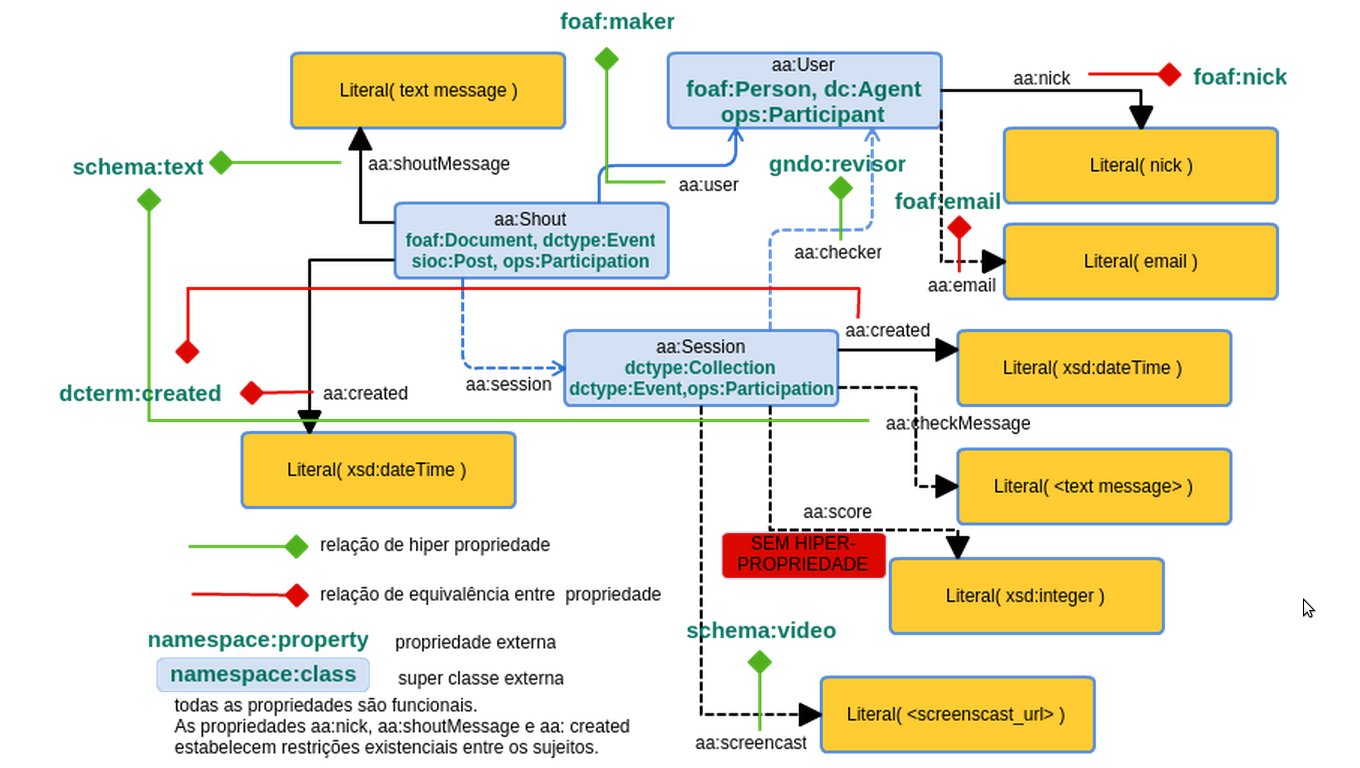
\includegraphics[width=\textwidth]{../figs/ontologiaa.png}
  \caption{Ontologia do AA, com suas classes, propriedades, literais, e classes e propriedades externas usadas para relacionar os dados do AA aos do participa e de toda nuvem LOD.}\label{fig:diaa}
\end{figure}

O tamanho reduzido da ontologia permitiu que vários testes fossem feitos. Em especial, com a ontologiaa foi reestabelecida a arquitetura de ontologia com uso de um namespace interno (no caso \url{http://purl.org/socialparticipation/aa/} e inferências para contemplar outros namespaces.

As inferências foram testadas com o jena/fuseki, com bons resultados. Tanto as inferências relacionadas às hiperonímias (superclasses e super propriedades, diretamente do rdfs) quanto inferências mais elaboradas (ligadas ao padrão OWL) foram satisfatórias. O revés é que qualquer query SparQL que demora milissegundos, mesmo que não envolva inferências para sua resposta, demora segundos quando há uma máquina de inferências ativa. A solução, portanto, parece ser ainda de realizar estas inferências offline e disponibilizar todas as triplas resultantes no endpoint.

Todos os desenvolvimentos desta ontologia e a triplificação de dados do AA em MySQL e MongoDB estão em: \url{https://github.com/ttm/aa01/tree/master/rdf}. Estes dados estão disponíveis no endpoint sparql (fuseki/jena) para uso conforme \url{script ipython}. Há interfaces úteis para explorar/expor os dados ligados ao AA. Em especial, estão derreferenciáveis, como na Figura~\ref{fig:aashout}.

\begin{figure}[h!]
  \centering
    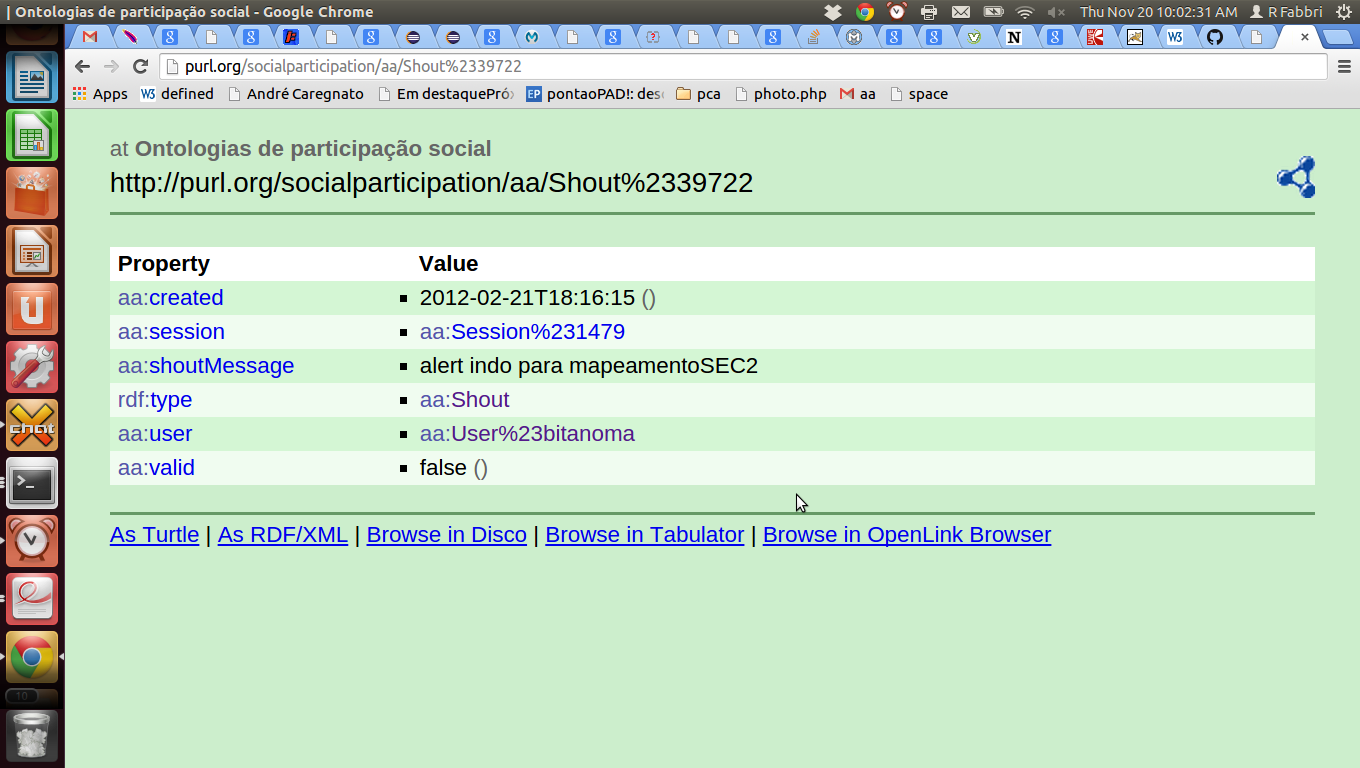
\includegraphics[width=\textwidth]{../figs/aaShoutPubby.png}
  \caption{Mensagem (shout) do AA derreferenciado. Cada mensagem do AA recebe uma URI, assim como cada sessão e cada usuário. Estes três conceitos são instânciados com URIs dedicadas, e relacionadas via ainda outras URIs. Por fim URIs especificam relações entre instâncias destes conceitos e os dados.}\label{fig:aashout}
\end{figure}

A ontologia do AA está no webprotege da Stanford~\url{http://webprotege.stanford.edu/#Edit:projectId=5207dd13-8706-4836-bad9-6cba1c81de29}.

\subsection{Ontologia do Cidade Democrática (OCD)}
Outra instância participativa considerada prioritária pelo consultor para integração aos dados participativos linkados, e contemplada neste trabalho, foi o portal Cidade Democrática. Este portal possui grande complexidade e abundância de dados e conceitos. Assim, esta empreitada contrastou com a da Ontologiaa descrito no Apêndice~\ref{ap:aa}.

Com a grande complexidade das tabelas e dados, foi feita uma decupagem do banco de dados (disponibilizada em \url{https://github.com/ttm/ocd/blob/master/decupagemBD.txt}) e uma triplificação destes dados (script em: \url{https://github.com/ttm/ocd/blob/master/triplificaCD.py} e triplas resultantes em \url{https://github.com/ttm/ocd/blob/master/cdTriplestore.rdf.tar.gz}).

Embora os trabalhos de decupagem do banco e de triplificação dos dados sejam expressivos, o ponto alto desta empreitada foi a gênese de um método de levantamento de ontologia orientado aos dados. Este método é extremamente útil para qualquer portal que queira representar seus dados como triplas RDF e uma ontologia. O processo é o seguinte:

\begin{enumerate}
    \item Todos os dados de interesse são triplificados com namespace interno, conforme: \url{https://github.com/ttm/ocd/blob/master/triplificaCD.py}.
    \item Os dados triplificados são disponibilizados em um endpoint sparql para levantamento da ontologia com base nas triplas produzidas (endpoint em: \url{http://200.144.255.210:8082/cd/query}).
    \item Um script é construído, no qual os dados triplificados são usados para observação das estruturas ocorrentes, conforme \url{https://github.com/ttm/ocd/blob/master/OCD.py}. Principalmente:
\begin{itemize}
        \item São observadas todas as classes ocorrentes.
        \item São observadas todas as propriedades ocorrentes.
        \item As propriedades são especificadas como funcionais e inversamente funcionais (axiomas de propriedade), conforme os dados apresentarem tais relações.
        \item As classes recebem restrições universais e existenciais, conforme os dados apresentarem estas relações.
        \item São feitas imagens de cada propriedade, com os elementos imediatamente relacionados a eles, como na Figura~\ref{fig:ocdp}.
        \item São feitas imagens de cada classe, com os elementos imediatamente relacionados a eles, como na Figura~\ref{fig:ocdc}.
        \item São feitas imagens diferentes da estrutura global, para facilitar apreensão da ontologia, como a Figura~\ref{fig:ocdg}.
        \item Ontologia OWL é escrita, conforme disponibilizada em: \url{https://github.com/ttm/ocd/blob/master/OCD.owl} ou \url{https://github.com/ttm/ocd/blob/master/OCD.ttl}.
        \item Os conceitos são relacionados a conceitos mais gerais, de ontologias externas, para facilitar a integração dos dados do portal com o grafo gigante e global~\cite{LOD}. Este passo não foi dado na OCD por limitação de tempo mesmo. Há outras prioridades e a comunidade deste portal está ainda absorvendo as informações e tecnologias disponibilizadas com este produto.
\end{itemize}
\end{enumerate}

Esta ontologia está no Webprotege disponibilizado pela Stanford, no link: \url{http://webprotege.stanford.edu/#Edit:projectId=a6e2334c-5c32-4397-9c9a-c75c1cebb555} com todas as classes e propriedades comentáveis. Digno de nota: o detalhamento nas restrições de classes e nos axiomas de propriedade, embora usualmente não recomendados com tanta extensão para não forçar aplicação menos rígida, permitem mais inferencias. Além disso, este detalhamento melhorou bastante a navegação da estrutura, como pode-se observar no próprio webprotege.

\begin{figure}[h!]
  \centering
    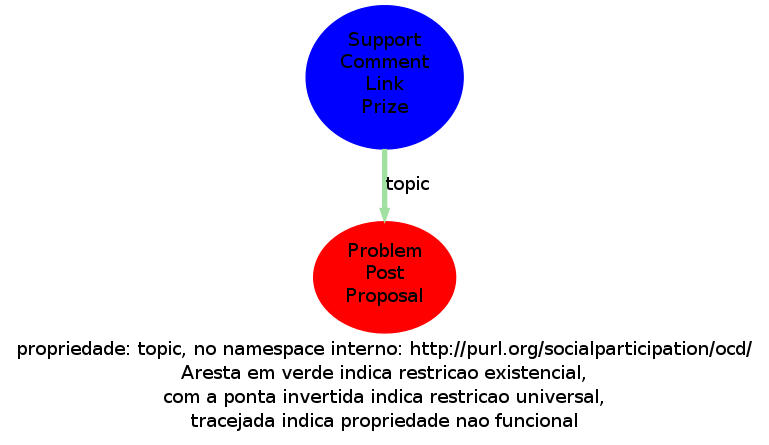
\includegraphics[width=\textwidth]{../figs/topic.png}
  \caption{Figura da propriedade \texttt{ocd:topic}, fruto do método de especificação de ontologias orientado aos dados.}\label{fig:ocdp}
\end{figure}

\begin{figure}[h!]
  \centering
    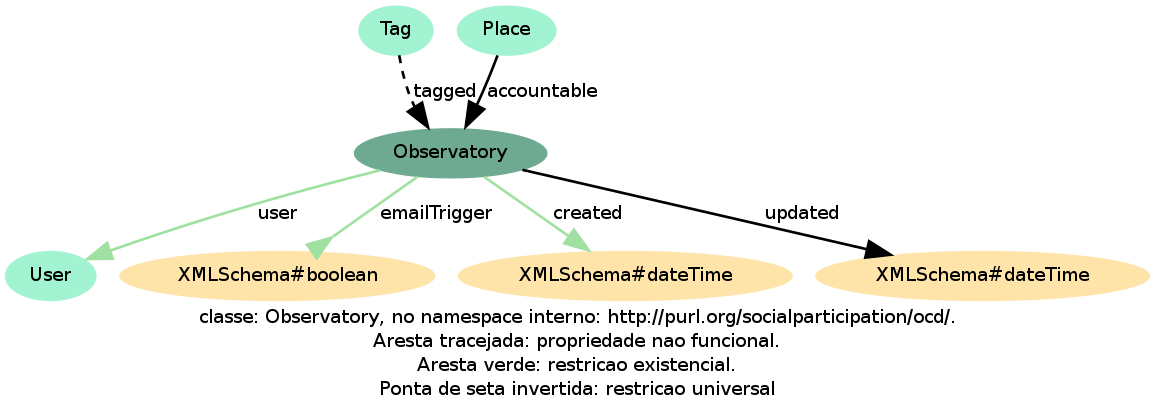
\includegraphics[width=\textwidth]{../figs/Observatory.png}
  \caption{Figura da classe \texttt{ocd:Observatory}, fruto do método de especificação de ontologias orientado aos dados.}\label{fig:ocdc}
\end{figure}

\begin{figure}[h!]
  \centering
    \includegraphics[width=\textwidth]{../figs/OCD_2.png}
  \caption{Figura geral da ontologia \texttt{ocd}, fruto do método de especificação de ontologias orientado aos dados. Para facilitar visualização, visite as imagens diretamente em~\url{https://raw.githubusercontent.com/ttm/ocd/master/imgs/OCD_.png} e~\url{https://raw.githubusercontent.com/ttm/ocd/master/imgs/OCD_2.png}.}\label{fig:ocdg}
\end{figure}


\section{Revisão da OPa}\label{ap:opa}
O primeiro produto desta consultoria envolveu o levantamento de uma ontologia para o Participa, batizada de OPa. Isso ocorreu antes de serem triplificados os dados do participa.br e antes até mesmo do consultor ter acesso a estes dados. Isso foi bastante proveitoso, pois obrigou a equipe do participa a conceber uma ontologia genérica para portais participativos, centrada nos conceitos de participante, portal participativo e mecanismo participativo. Estes módulos estarão preservados e constam como legado intelectual, uma contribuição da equipe do participa.br na conceituação da participação social online.

Já depois de feitas estas ontologias do AA e do Cidade Democrática, e depois de ter feito toda a OBS e VBS, atingimos um paradigma apropriado para triplificação dos dados e organização conceitual. Em resumo:
\begin{itemize}
    \item uso de um namespace interno, como \texttt{http://purl.org/socialparticipation/opa}, para a triplificação dos dados, em todas as classes e propriedades. Isso facilita a navegacao e deixa os dados mais organizados, pois no caso extremo de compatibilidade com alguma classe externa, a classe interna assinala a fonte da instância. Um caso extremo desta pertinência é com o derreferenciamento, em que a url \url{http://purl.org/socialparticipation/opa/Participant} lista todos os participantes da OPA, e sua superclasse, \url{http://purl.org/socialparticipation/ops/Participant} apresenta todos os participantes, sejam da OPA, do AA ou do Cidade Democrática.
    \item Relacionamento das triplas com namespaces externos através da ontologia, com as propriedades \texttt{rdfs:subClassOf} e~\texttt{rdfs:subPropertyOf}. Esta implementação pode vir na medida em que a comunidade se apropriar do andamento, pois estas inferências tornam as consultas lentas pela utilização da máquina de inferência em tempo real ou aumentam a quantidade de triplas no caso das inferências offline. Ou seja, nos estágios iniciais, é mais leve e simples não utilizar namespaces externos.
    \item Liberação da ontologia com \emph{blueprints} em imagens. Acréscimo das restrições de classe, e axiomas de pripriedade na medida em que houver utilidade para não enrijecer a estrutura.
\end{itemize}

Neste contexto, além da ontologia disponível no primeiro produto desta consultoria, a OPa conta com as estruturas orientadas aos dados do portal, apresentadas nas imagens~\ref{fig:},~\ref{fig:},~\ref{fig:}.

\section{Revisão da Triplificação do Participa.br}
O script de triplificação disponibilizado no produto 2 foi adaptado para o paradigma explicitado no Apêndice~\ref{ap:ropa}. Além disso,
foram acrescentadas à triplificação algumas informações adicionais de usuários e das postagens em si. O script de triplificação, revisado, está em: \url{http://github.com/ttm/pnud5/scripts/triplificaParticipa22112014.py}.

\section{Ontologia e Vocabulário da Biblioteca Social (OBS e VBS)}
Por ocasião do levantamento da Biblioteca (digital e semântica de participação) Social, por iniciativa da SNAS/SGPR e com esforços de diversos parceiros, o consultor iniciou uma sequência de entrevistas que culminaram com um workshop na SGPR no dia 20/10/2014, para contribuições de parceiros diversos. Além das entrevistas individuais e dos workshops, foram consideradas documentações de referência produzidas sobre e pelos mecanismos e instancias de participação social. A PNPS foi considerada separadamente, dado o monumento informacional que contém o decreto. Todo o processo foi permeado de diversas trocas de mensagens entre o consultor e equipes do particpa.br, UnB, IPEA, SNAS e MP.

Este apêndice expõe estas contribuições e as resultantes organizações ontológicas e de vocabulários.

\subsection{Materiais enviados pela equipe para referência}
Foi considerado um material fruto de articulação da SNAS. O material consiste de documentos produzidos ou referentes às instâncias e mecanismos de participação social e um produto da consultora Carmen Romcy. Este material deu origem a um vocabulário SKOS sobre documentos de participação social, complementar aos obtidos nos apêndices seguintes. O script que escreve o SKOS em RDF/XML e Turtle está em: \url{://github.com/ttm/vocabulario-participacao/blob/master/scripts/vbsDocumentacaoVBS.py}. O RDF/XML em~\url{https://github.com/ttm/vocabulario-participacao/blob/master/rdf/vbsDocumentacaoVBS.rdf} e o Turtle em~\url{https://github.com/ttm/vocabulario-participacao/blob/master/rdf/vbsDocumentacaoVBS.ttl}. Em texto detalhado e em árvore taxonomica~\url{https://github.com/ttm/vocabulario-participacao/blob/master/txt/vbsDocumentacaoVBS.txt}, em texto corrido~\url{https://github.com/ttm/vocabulario-participacao/blob/master/txt/vbsDocumentacaoVBSPalavras.txt}.

O material em si está no link~\url{https://drive.google.com/file/d/0B7GnkNzm0kxvSTZWWDRyTFkzNm8/view?usp=sharing}.
 O decreto 8.243 é considerado no Apêndice~\ref{ap:pnps}.

\subsection{Entrevistas individuais}
Especialistas foram entrevistados para especificações ontológicas iniciais de instâncias de participação social. Os especialistas estão citados abaixo junto ao auxílio que prestaram.

\subsubsection{Especificação das Conferências - Clovis Souza}
Materiais iniciais dos profs. Fernando Cruz e Carmem Romcy permitiram rascunhos iniciais da ontologia de conferências nacionais. Estes rascunhos foram usados como base para a entrevista feita com o Clovis Souza. No dia 30/setembro e no dia 03/outubro, foram revisados os rascunhos iniciais e especificadas relações dos documentos. Foram gerados dois conjuntos de conceitos relacionados ontologicamente e com vocabulário.

O primeiro conjunto é centrado na conferência em si, e os conceitos principais envolvidos. O script que sintetiza o OWL em RDF/XML e Turtle, sintetiza 3 imagens da rede de conceitos (blueprint), e grava o arquivo .dot do grafo resultante está em~\url{https://github.com/ttm/vocabulario-participacao/blob/master/scripts/obsConferencias.py}. O RDF/XML está em \url{https://github.com/ttm/vocabulario-participacao/blob/master/rdf/obsConferencia.owl} e o Turtle em \url{https://github.com/ttm/vocabulario-participacao/blob/master/rdf/obsConferenciaDocsRes.ttl}. As imagens estão em~\url{https://github.com/ttm/vocabulario-participacao/raw/master/figs/obsConferencia.png},~\url{https://github.com/ttm/vocabulario-participacao/raw/master/figs/obsConferencia2.png},~\url{https://github.com/ttm/vocabulario-participacao/raw/master/figs/obsConferencia3.png}. O grafo em .dot (usado pelo está em

O segundo conjunto é centrado nos documentos e nos resultados de conferência.  O script que sintetiza o OWL em RDF/XML e Turtle, sintetiza 3 imagens da rede de conceitos (blueprint), e grava o arquivo .dot do grafo resultante está em~\url{https://github.com/ttm/vocabulario-participacao/blob/master/scripts/obsConferencias.py}.

% Fazer tabela para os links dos arquivos da OBS e VBS.

\begin{table}[htpq!]
\centering
\caption{Tabela de arquivos da OBS e VBS.}
\begin{tabular}{| p{6cm} | c | c | c | c | }\hline
 {\bf descrição} & {\bf script} & {\bf RDF/XML} & {\bf Turtle} & {\bf diagramas ou listagens} \\\hline\hline
vocabulário SKOS do material de referência enviado pela SNAS  & \ref{i:1} & \ref{i:2} & \ref{i:3} & \ref{i:4},~\ref{i:4_1},~\ref{i:5} \\\hline\hline
ontologia OWL das conferências (Clovis) &~\ref{i:6}&~\ref{i:7}&~\ref{i:8}&~\ref{i:9},~\ref{i:10},~\ref{i:11},~\ref{i:11_1} \\
vocabulário SKOS das conferências (Clovis) &~\ref{i:12}&~\ref{i:13}&~\ref{i:14}&~\ref{i:16},~\ref{i:17},~\ref{i:18} \\\hline\hline

ontologia OWL  de documentos e resultados das conferências (Clovis) &~\ref{i:6a}&~\ref{i:7a}&~\ref{i:8a}&~\ref{i:9a},~\ref{i:10a},~\ref{i:11a},~\ref{i:11_1a} \\
vocabulário SKOS de documentos e resultados das conferências (Clovis) &~\ref{i:12a}&~\ref{i:13a}&~\ref{i:14a}&~\ref{i:16a},~\ref{i:17a},~\ref{i:18a} \\\hline\hline

ontologia OWL dos conselhos (Paula) &~\ref{i:19}&~\ref{i:20}&~\ref{i:21}&~\ref{i:22},~\ref{i:23},~\ref{i:24},~\ref{i:24_1} \\
vocabulário SKOS dos conselhos (Paula) &~\ref{i:25}&~\ref{i:26}&~\ref{i:27}&~\ref{i:28},~\ref{i:29},~\ref{i:30} \\\hline\hline

ontologia   OWL das  ouvidorias (Lígia) &~\ref{i:31}&~\ref{i:32}&~\ref{i:33}&~\ref{i:34},~\ref{i:35},~\ref{i:36},~\ref{i:37} \\
vocabulário SKOS das ouvidorias (Lígia) &~\ref{i:38}&~\ref{i:39}&~\ref{i:40}&~\ref{i:41},~\ref{i:42},~\ref{i:43} \\\hline\hline

ontologia   OWL  das consultas públicas (XX) &~\ref{i:44}&~\ref{i:45}&~\ref{i:46}&~\ref{i:47},~\ref{i:48},~\ref{i:49},~\ref{i:50} \\
vocabulário SKOS das consultas públicas (XX) &~\ref{i:51}&~\ref{i:52}&~\ref{i:53}&~\ref{i:54},~\ref{i:55},~\ref{i:56} \\\hline\hline

ontologia   OWL  das mesas de diálogo (XX) &~\ref{i:57}&~\ref{i:58}&~\ref{i:59}&~\ref{i:60},~\ref{i:61},~\ref{i:62},~\ref{i:63} \\
vocabulário SKOS das mesas de diálogo (XX) &~\ref{i:64}&~\ref{i:65}&~\ref{i:66}&~\ref{i:67},~\ref{i:68},~\ref{i:69} \\\hline\hline

ontologia   OWL  do Decreto 8.243 (PNPS) &~\ref{i:70}&~\ref{i:71}&~\ref{i:72}&~\ref{i:73},~\ref{i:74},~\ref{i:76} \\
vocabulário SKOS do Decreto 8.243 (PNPS) &~\ref{i:77}&~\ref{i:78}&~\ref{i:79}&~\ref{i:80},~\ref{i:81},~\ref{i:82} \\\hline\hline

vocabulário SKOS do Vocabulário do IPEA de Participação Social &~\ref{i:83}&~\ref{i:84}&~\ref{i:85}&~\ref{i:86} \\\hline\hline


\end{tabular}\label{eq:intervalos}
\end{table}

Links:
{\scriptsize
\begin{enumerate}
    \item \url{https://raw.githubusercontent.com/ttm/vocabulario-participacao/master/scripts/vbsDocumentacaoVBS.py}\label{i:1}
    \item \url{https://raw.githubusercontent.com/ttm/vocabulario-participacao/master/rdf/vbsDocumentacaoVBS.rdf}\label{i:2}
    \item \url{https://raw.githubusercontent.com/ttm/vocabulario-participacao/master/rdf/vbsDocumentacaoVBS.ttl}\label{i:3}
    \item \url{https://raw.githubusercontent.com/ttm/vocabulario-participacao/master/txt/vbsDocumentacaoVBS.txt} \label{i:4}
    \item \url{https://raw.githubusercontent.com/ttm/vocabulario-participacao/master/txt/vbsDocumentacaoVBSPodada.txt}\label{i:4_1}
    \item \url{https://raw.githubusercontent.com/ttm/vocabulario-participacao/master/txt/vbsDocumentacaoVBSPalavras.txt}\label{i:5}

    \item \url{https://raw.githubusercontent.com/ttm/vocabulario-participacao/master/scripts/obsConferencias.py}\label{i:6}
    \item \url{https://raw.githubusercontent.com/ttm/vocabulario-participacao/master/rdf/obsConferencia.owl}\label{i:7}
    \item \url{https://raw.githubusercontent.com/ttm/vocabulario-participacao/master/rdf/obsConferencia.ttl}\label{i:8}
    \item \url{https://raw.githubusercontent.com/ttm/vocabulario-participacao/master/figs/obsConferencia.png}\label{i:9}
    \item \url{https://raw.githubusercontent.com/ttm/vocabulario-participacao/master/figs/obsConferencia.png}\label{i:10}
    \item \url{https://raw.githubusercontent.com/ttm/vocabulario-participacao/master/figs/obsConferencia.png}\label{i:11}
    \item \url{https://raw.githubusercontent.com/ttm/vocabulario-participacao/master/dot/obsConferencia.dot}\label{i:11_1}

    \item \url{https://raw.githubusercontent.com/ttm/vocabulario-participacao/master/scripts/vbsConferencias.py}\label{i:12}
    \item \url{https://raw.githubusercontent.com/ttm/vocabulario-participacao/master/rdf/vbsConferencia.rdf}\label{i:13}
    \item \url{https://raw.githubusercontent.com/ttm/vocabulario-participacao/master/rdf/vbsConferencia.ttl}\label{i:14}
    \item \url{https://raw.githubusercontent.com/ttm/vocabulario-participacao/master/txt/vbsConferencia.txt}\label{i:16}
    \item \url{https://raw.githubusercontent.com/ttm/vocabulario-participacao/master/txt/vbsConferenciaPalavras.txt}\label{i:17}
    \item \url{https://raw.githubusercontent.com/ttm/vocabulario-participacao/master/txt/vbsConferenciaPodada.txt}\label{i:18}

 \item \url{https://raw.githubusercontent.com/ttm/vocabulario-participacao/master/scripts/obsConferenciasDocsRes.py}    \label{i:6a}
     \item \url{https://raw.githubusercontent.com/ttm/vocabulario-participacao/master/rdf/obsConferenciaDocsRes.owl}    \label{i:7a}
     \item \url{https://raw.githubusercontent.com/ttm/vocabulario-participacao/master/rdf/obsConferenciaDocsRes.ttl}    \label{i:8a}
    \item \url{https://raw.githubusercontent.com/ttm/vocabulario-participacao/master/figs/obsConferenciaDocsRes.png}    \label{i:9a}
    \item \url{https://raw.githubusercontent.com/ttm/vocabulario-participacao/master/figs/obsConferenciaDocsRes.png}   \label{i:10a}
    \item \url{https://raw.githubusercontent.com/ttm/vocabulario-participacao/master/figs/obsConferenciaDocsRes.png}   \label{i:11a}
     \item \url{https://raw.githubusercontent.com/ttm/vocabulario-participacao/master/dot/obsConferenciaDocsRes.dot} \label{i:11_1a}

\item \url{https://raw.githubusercontent.com/ttm/vocabulario-participacao/master/scripts/vbsConferenciasDocsRes.py}         \label{i:12a}
     \item \url{https://raw.githubusercontent.com/ttm/vocabulario-participacao/master/rdf/vbsConferenciaDocsRes.rdf}        \label{i:13a}
     \item \url{https://raw.githubusercontent.com/ttm/vocabulario-participacao/master/rdf/vbsConferenciaDocsRes.ttl}        \label{i:14a}
     \item \url{https://raw.githubusercontent.com/ttm/vocabulario-participacao/master/txt/vbsConferenciaDocsRes.txt}        \label{i:16a}
     \item \url{https://raw.githubusercontent.com/ttm/vocabulario-participacao/master/txt/vbsConferenciaDocsResPalavras.txt}\label{i:17a}
     \item \url{https://raw.githubusercontent.com/ttm/vocabulario-participacao/master/txt/vbsConferenciaDocsResPodada.txt}  \label{i:18a}



    \item \url{https://raw.githubusercontent.com/ttm/vocabulario-participacao/master/scripts/obsConselhos.py}\label{i:19}
    \item  \url{https://raw.githubusercontent.com/ttm/vocabulario-participacao/master/rdf/obsConselho.owl}\label{i:20}
    \item  \url{https://raw.githubusercontent.com/ttm/vocabulario-participacao/master/rdf/obsConselho.ttl}\label{i:21}
    \item \url{https://raw.githubusercontent.com/ttm/vocabulario-participacao/master/figs/obsConselho.png}\label{i:22}
    \item \url{https://raw.githubusercontent.com/ttm/vocabulario-participacao/master/figs/obsConselho.png}\label{i:23}
    \item \url{https://raw.githubusercontent.com/ttm/vocabulario-participacao/master/figs/obsConselho.png}\label{i:24}
    \item \url{https://raw.githubusercontent.com/ttm/vocabulario-participacao/master/dot/obsConselho.dot}\label{i:24_1}

    \item \url{https://raw.githubusercontent.com/ttm/vocabulario-participacao/master/scripts/vbsConselhos.py}\label{i:25}
    \item \url{https://raw.githubusercontent.com/ttm/vocabulario-participacao/master/rdf/vbsConselho.rdf}\label{i:26}
    \item \url{https://raw.githubusercontent.com/ttm/vocabulario-participacao/master/rdf/vbsConselho.ttl}\label{i:27}
    \item \url{https://raw.githubusercontent.com/ttm/vocabulario-participacao/master/txt/vbsConselho.txt}\label{i:28}
    \item \url{https://raw.githubusercontent.com/ttm/vocabulario-participacao/master/txt/vbsConselhoPalavras.txt}\label{i:29}
    \item \url{https://raw.githubusercontent.com/ttm/vocabulario-participacao/master/txt/vbsConselhoPodada.txt}\label{i:30}

    \item \url{https://raw.githubusercontent.com/ttm/vocabulario-participacao/master/scripts/obsOuvidorias.py}\label{i:31}
    \item  \url{https://raw.githubusercontent.com/ttm/vocabulario-participacao/master/rdf/obsOuvidoria.owl}\label{i:32}
    \item  \url{https://raw.githubusercontent.com/ttm/vocabulario-participacao/master/rdf/obsOuvidoria.ttl}\label{i:33}
    \item \url{https://raw.githubusercontent.com/ttm/vocabulario-participacao/master/figs/obsOuvidoria.png}\label{i:34}
    \item \url{https://raw.githubusercontent.com/ttm/vocabulario-participacao/master/figs/obsOuvidoria.png}\label{i:35}
    \item \url{https://raw.githubusercontent.com/ttm/vocabulario-participacao/master/figs/obsOuvidoria.png}\label{i:36}
    \item  \url{https://raw.githubusercontent.com/ttm/vocabulario-participacao/master/dot/obsOuvidoria.dot}\label{i:37}

    \item \url{https://raw.githubusercontent.com/ttm/vocabulario-participacao/master/scripts/vbsOuvidorias.py}\label{i:38}
    \item \url{https://raw.githubusercontent.com/ttm/vocabulario-participacao/master/rdf/vbsOuvidoria.rdf}\label{i:39}
    \item \url{https://raw.githubusercontent.com/ttm/vocabulario-participacao/master/rdf/vbsOuvidoria.ttl}\label{i:40}
    \item \url{https://raw.githubusercontent.com/ttm/vocabulario-participacao/master/txt/vbsOuvidoria.txt}\label{i:41}
    \item \url{https://raw.githubusercontent.com/ttm/vocabulario-participacao/master/txt/vbsOuvidoriaPalavras.txt}\label{i:42}
    \item \url{https://raw.githubusercontent.com/ttm/vocabulario-participacao/master/txt/vbsOuvidoriaPodada.txt}\label{i:43}


 \item \url{https://raw.githubusercontent.com/ttm/vocabulario-participacao/master/scripts/obsConsultas.py}\label{i:44}
    \item  \url{https://raw.githubusercontent.com/ttm/vocabulario-participacao/master/rdf/obsConsulta.owl}\label{i:45}
    \item  \url{https://raw.githubusercontent.com/ttm/vocabulario-participacao/master/rdf/obsConsulta.ttl}\label{i:46}
    \item \url{https://raw.githubusercontent.com/ttm/vocabulario-participacao/master/figs/obsConsulta.png}\label{i:47}
    \item \url{https://raw.githubusercontent.com/ttm/vocabulario-participacao/master/figs/obsConsulta.png}\label{i:48}
    \item \url{https://raw.githubusercontent.com/ttm/vocabulario-participacao/master/figs/obsConsulta.png}\label{i:49}
    \item  \url{https://raw.githubusercontent.com/ttm/vocabulario-participacao/master/dot/obsConsulta.dot}\label{i:50}

\item \url{https://raw.githubusercontent.com/ttm/vocabulario-participacao/master/scripts/vbsConsultas.py}        \label{i:51}
    \item \url{https://raw.githubusercontent.com/ttm/vocabulario-participacao/master/rdf/vbsConsulta.rdf}        \label{i:52}
    \item \url{https://raw.githubusercontent.com/ttm/vocabulario-participacao/master/rdf/vbsConsulta.ttl}        \label{i:53}
    \item \url{https://raw.githubusercontent.com/ttm/vocabulario-participacao/master/txt/vbsConsulta.txt}        \label{i:54}
    \item \url{https://raw.githubusercontent.com/ttm/vocabulario-participacao/master/txt/vbsConsultaPalavras.txt}\label{i:55}
    \item \url{https://raw.githubusercontent.com/ttm/vocabulario-participacao/master/txt/vbsConsultaPodada.txt}  \label{i:56}

 \item \url{https://raw.githubusercontent.com/ttm/vocabulario-participacao/master/scripts/obsMesasDeDialogo.py}\label{i:57}
    \item  \url{https://raw.githubusercontent.com/ttm/vocabulario-participacao/master/rdf/obsMesaDeDialogo.owl}\label{i:58}
    \item  \url{https://raw.githubusercontent.com/ttm/vocabulario-participacao/master/rdf/obsMesaDeDialogo.ttl}\label{i:59}
    \item \url{https://raw.githubusercontent.com/ttm/vocabulario-participacao/master/figs/obsMesaDeDialogo.png}\label{i:60}
    \item \url{https://raw.githubusercontent.com/ttm/vocabulario-participacao/master/figs/obsMesaDeDialogo.png}\label{i:61}
    \item \url{https://raw.githubusercontent.com/ttm/vocabulario-participacao/master/figs/obsMesaDeDialogo.png}\label{i:62}
    \item  \url{https://raw.githubusercontent.com/ttm/vocabulario-participacao/master/dot/obsMesaDeDialogo.dot}\label{i:63}

\item \url{https://raw.githubusercontent.com/ttm/vocabulario-participacao/master/scripts/vbsMesasDeDialogo.py}        \label{i:64}
    \item \url{https://raw.githubusercontent.com/ttm/vocabulario-participacao/master/rdf/vbsMesaDeDialogo.rdf}        \label{i:65}
    \item \url{https://raw.githubusercontent.com/ttm/vocabulario-participacao/master/rdf/vbsMesaDeDialogo.ttl}        \label{i:66}
    \item \url{https://raw.githubusercontent.com/ttm/vocabulario-participacao/master/txt/vbsMesaDeDialogo.txt}        \label{i:67}
    \item \url{https://raw.githubusercontent.com/ttm/vocabulario-participacao/master/txt/vbsMesaDeDialogoPalavras.txt}\label{i:68}
    \item \url{https://raw.githubusercontent.com/ttm/vocabulario-participacao/master/txt/vbsMesaDeDialogoPodada.txt}  \label{i:69}

 \item \url{https://raw.githubusercontent.com/ttm/vocabulario-participacao/master/scripts/obsPNPS.py} \label{i:70}
    \item  \url{https://raw.githubusercontent.com/ttm/vocabulario-participacao/master/rdf/obsPNPS.owl}\label{i:71}
    \item  \url{https://raw.githubusercontent.com/ttm/vocabulario-participacao/master/rdf/obsPNPS.ttl}\label{i:72}
    \item \url{https://raw.githubusercontent.com/ttm/vocabulario-participacao/master/figs/obsPNPS.png}\label{i:73}
    \item \url{https://raw.githubusercontent.com/ttm/vocabulario-participacao/master/figs/obsPNPS3.png}\label{i:75}
    \item  \url{https://raw.githubusercontent.com/ttm/vocabulario-participacao/master/dot/obsPNPS.dot}\label{i:76}

\item \url{https://raw.githubusercontent.com/ttm/vocabulario-participacao/master/scripts/vbsPNPS.py}         \label{i:77}
    \item \url{https://raw.githubusercontent.com/ttm/vocabulario-participacao/master/rdf/vbsPNPS.rdf}        \label{i:78}
    \item \url{https://raw.githubusercontent.com/ttm/vocabulario-participacao/master/rdf/vbsPNPS.ttl}        \label{i:79}
    \item \url{https://raw.githubusercontent.com/ttm/vocabulario-participacao/master/txt/vbsPNPS.txt}        \label{i:80}
    \item \url{https://raw.githubusercontent.com/ttm/vocabulario-participacao/master/txt/vbsPNPSPalavras.txt}\label{i:81}
    \item \url{https://raw.githubusercontent.com/ttm/vocabulario-participacao/master/txt/vbsPNPSPodada.txt}  \label{i:82}

\item \url{https://raw.githubusercontent.com/ttm/vocabulario-participacao/master/scripts/vbsIPEA.py}         \label{i:83}
    \item \url{https://raw.githubusercontent.com/ttm/vocabulario-participacao/master/rdf/vbsIPEA.rdf}        \label{i:84}
    \item \url{https://raw.githubusercontent.com/ttm/vocabulario-participacao/master/rdf/vbsIPEA.ttl}        \label{i:85}
    \item \url{https://raw.githubusercontent.com/ttm/vocabulario-participacao/master/txt/vbsIPEAPalavras.txt}\label{i:86}



\end{enumerate}
}



\subsection{Relatório de implementação das contribuições do Workshop dia 20/Out/2014, sobre a biblioteca (semântica de participação) social}
\begin{figure}[h!]
  \centering
    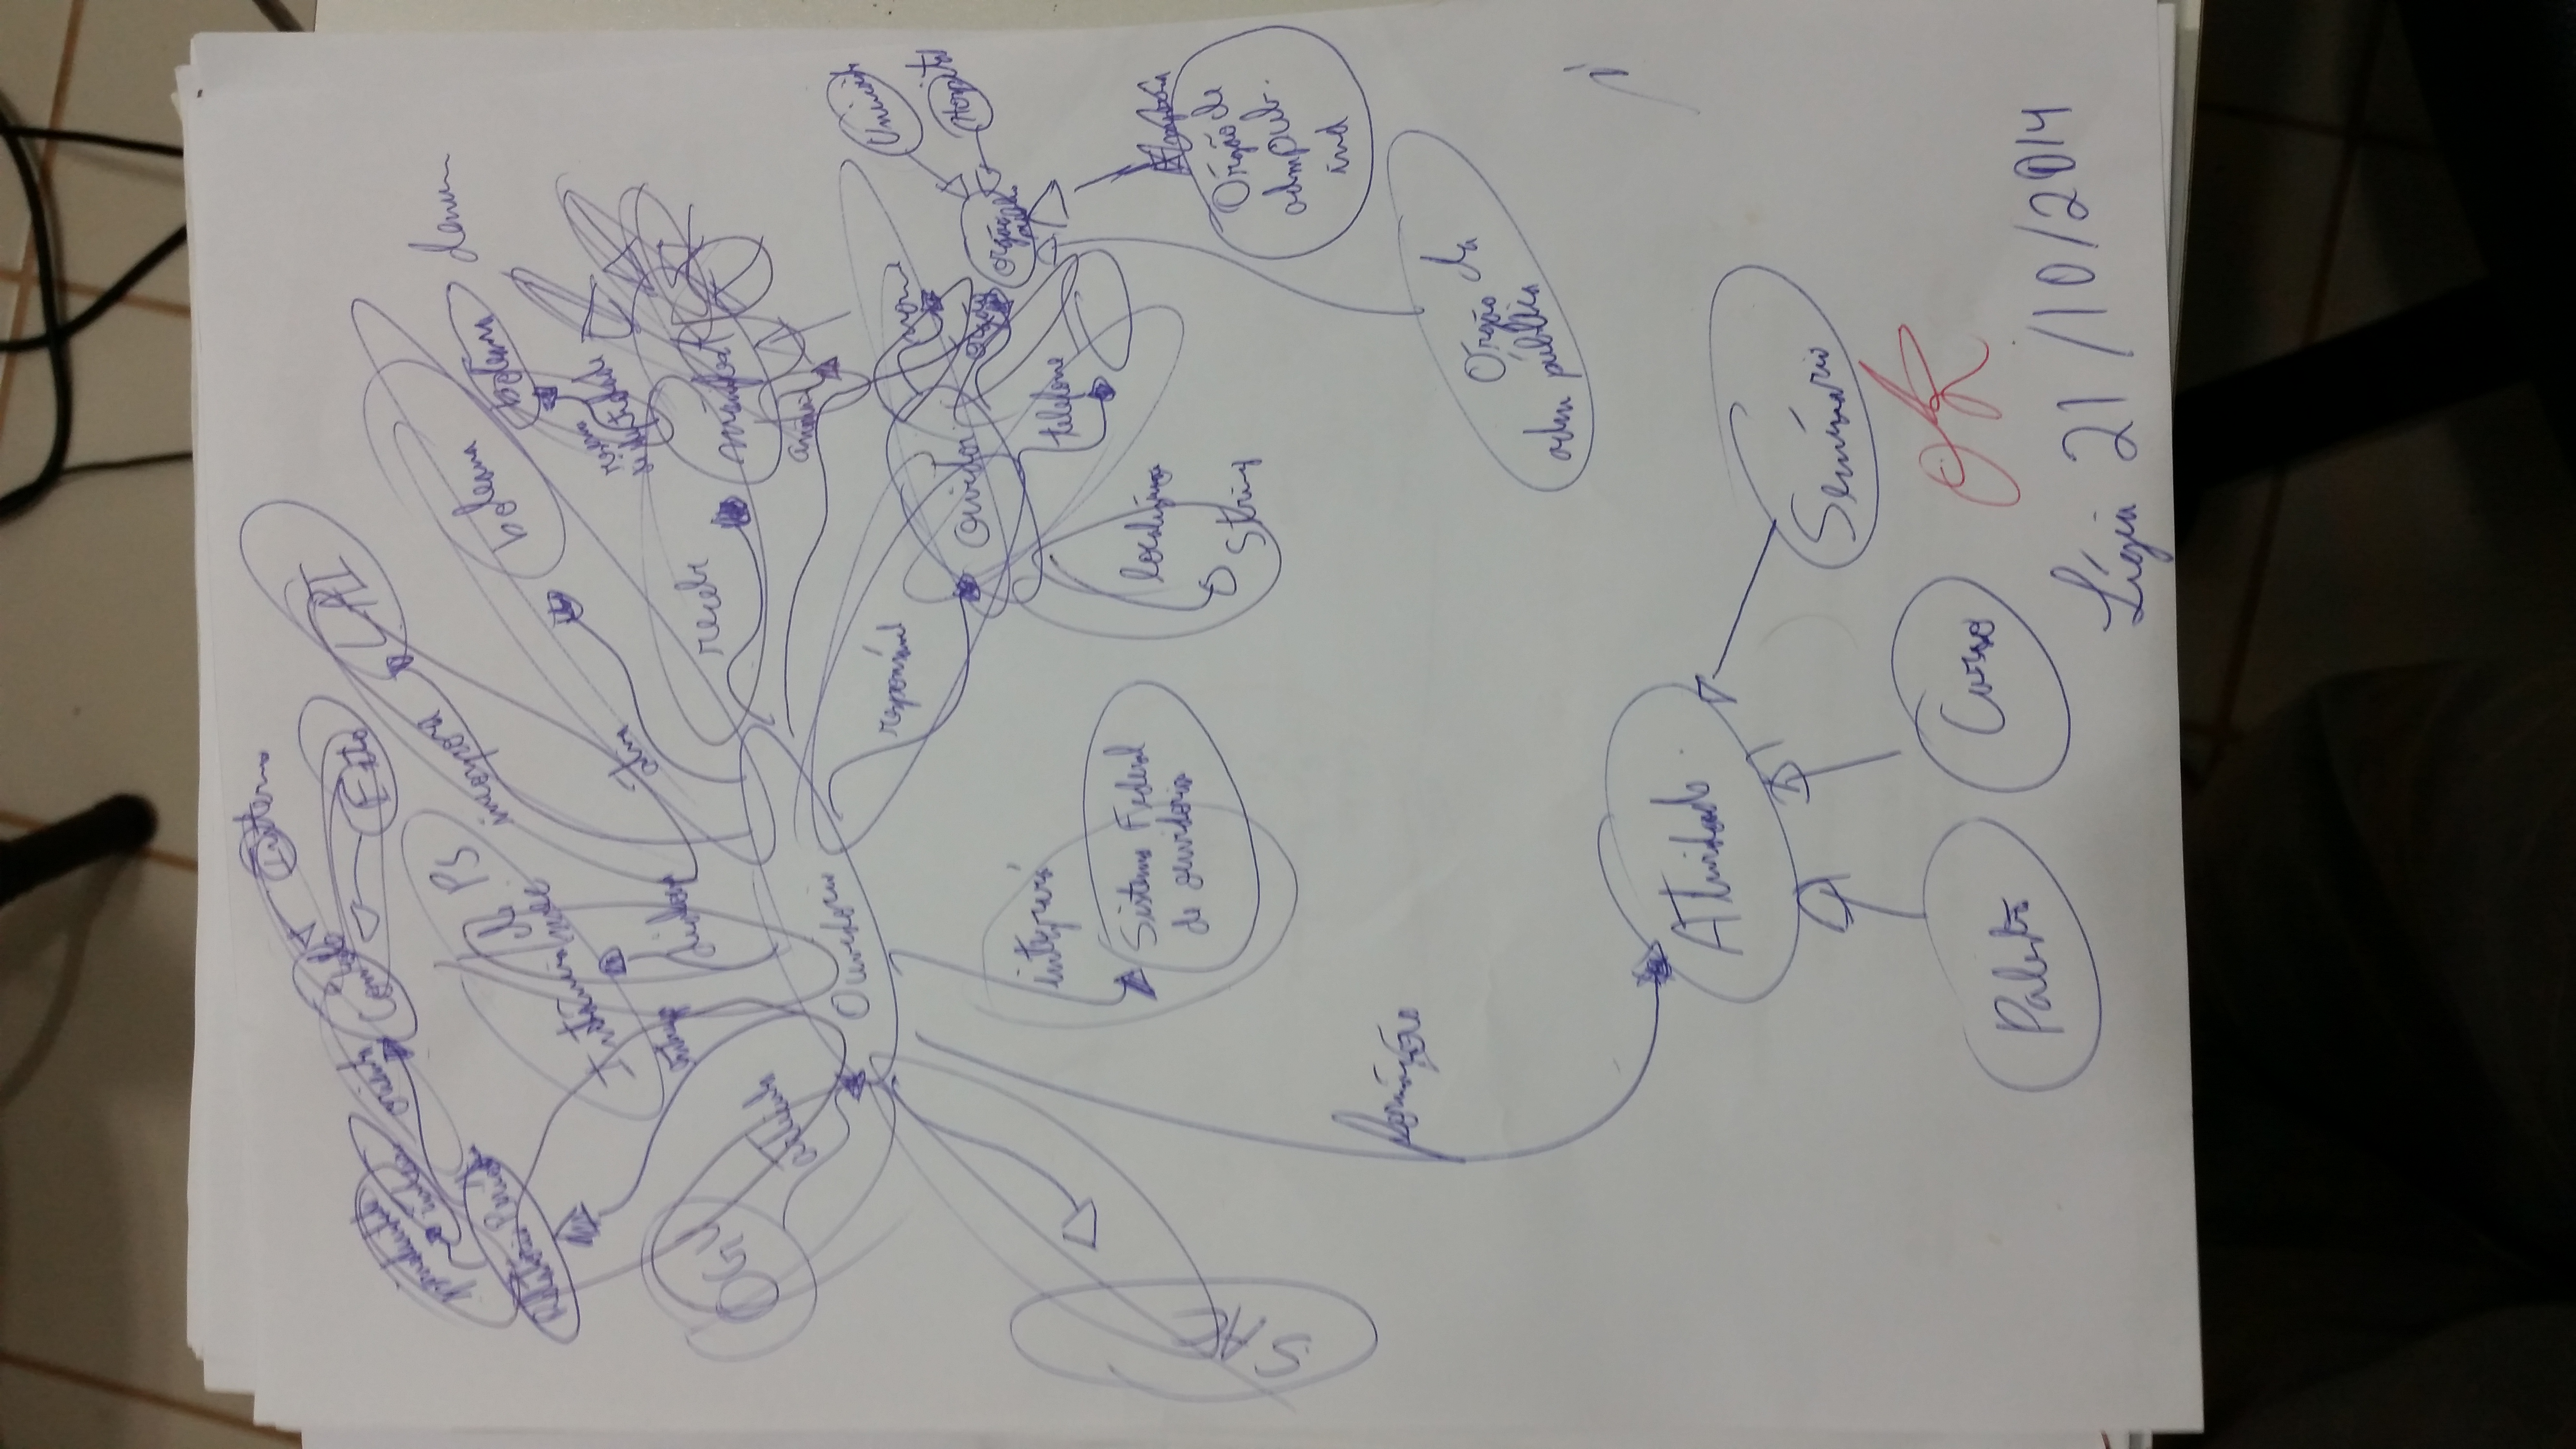
\includegraphics[width=\textwidth,angle=270]{fotos/OuvidoriaLigia.jpg}
  \caption{Diagrama de Ouvidorias desenhado com o acompanhamento de especialista (Lígia).}
\end{figure}
\subsection{PNPS}\label{ap:pnps}
 e a própria PNPS.

\section{Utilização dos dados linkados}

As ontologias mais importantes para este trabalho precisam ser observáveis e anotáveis com facilidade por não especialistas.

Uma primeira opção é aproveitar os dados/tripas disponíveis no endpoint sparql já aberto com uma instância Fuseki/Jena. Este endpoint pode ser acessado via linguagens de scripting para prototipação rápida, como JavaScript ou Python, fornecendo interfaces gráficas e web para navegação e análise. Estas possibilidades estão desenvolvidas nos produtos 2 e 3 desta mesma consultoria~\cite{prod2, prod3}.

\subsection{Pubby}

Com desenvolvimento recente no github \url{https://github.com/cygri/pubby}, é talvez o navegador de dados mais conhecido. Parece ser projeto do dig (grupo do Berners-Lee no MIT).
Os testes mostraram que as consultas sparql demoravam demais para o montante de dados triplificados, portanto foram importados os rdfs. Para facilitar, o arquivo de configuração do pubby está em \url{https://github.com/ttm/vocabulario-participacao/blob/master/auxiliar/config.ttl}.

A url permanente \url{http://purl.org/socialparticipation/} é redirecionada para a instância do pubby, em: \url{http://200.144.255.210:8081/tpubby/page/}. Desta forma, \emph{todos} os conceitos da VBS e classes da OBS podem ser derreferenciados, como na Figura~\ref{fig:derre}.

\begin{figure}[h!]
  \centering
    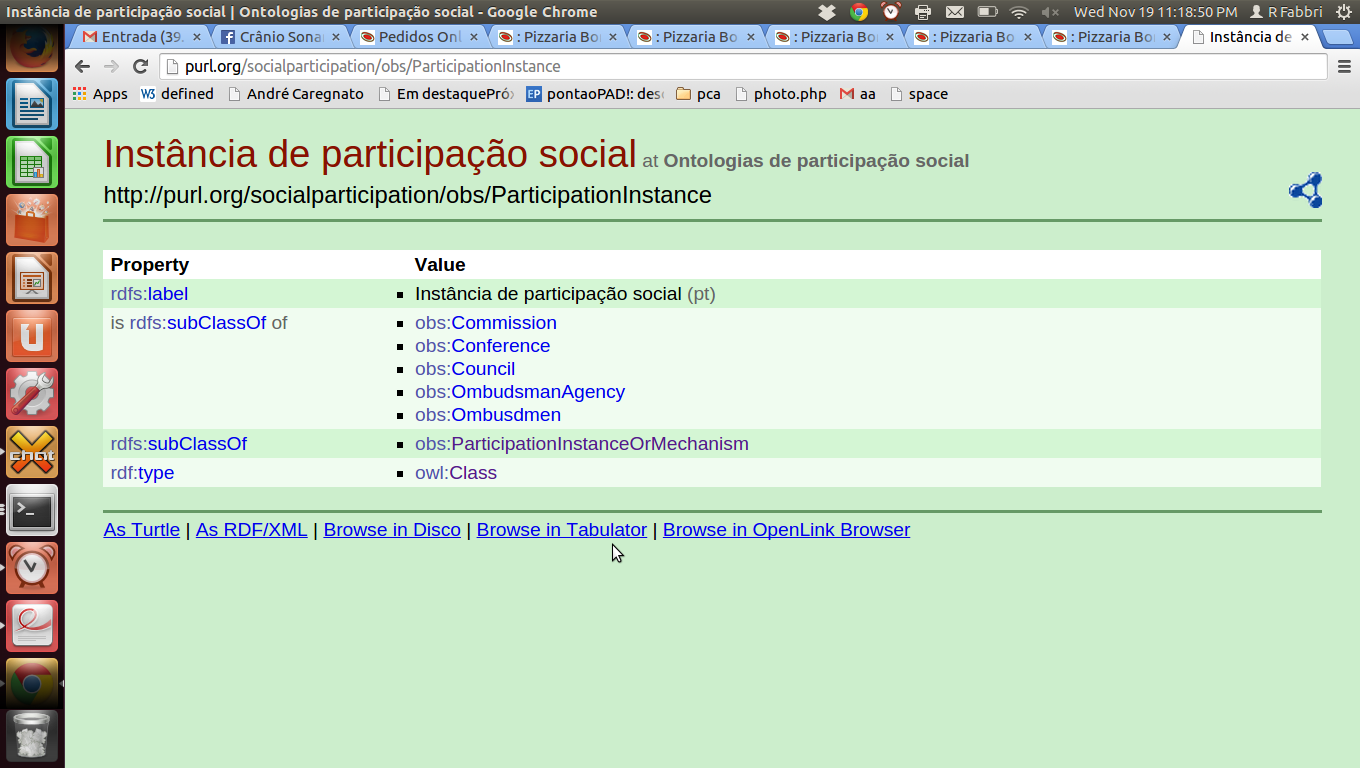
\includegraphics[width=\textwidth]{../figs/derre.png}
  \caption{Derreferenciamento do conceito de Instância de participação através da URI \url{http://purl.org/socialparticipation/obs/ParticipationInstance}.}\label{fig:derre}
\end{figure}

\subsection{Endpoint SparQL}

Os dados da OBS, VBS, Participabr, AA e OCD estão disponíveis via endpoint SparQL, conforme o uso explicitado nos scripts do INotebook \url{http://200.144.255.210:8003/}.

\subsection{Webprotege}

Permite que as ontologias e vocabulários estejam online e comentáveis.

%\section{Cartas ao poder público federal}
%\subsection{Religião e cultura livre}
%\subsection{Autoritarismo/preconceito e rede social}
%\subsection{Pesquisa e desenvolvimento para participação}
%\subsection{Subsídios para pulverizar a participação e qualificá-la}

%\section{Técnicas de difusão de informação}
%\subsection{Reprodução do experimento apocalíptico de 2012}




\end{document}
